% !TEX root = task-3-19-4.tex
% Editable task bank. Append new BankTask blocks at the end of the document.
\documentclass[12pt,a4paper]{article}
\usepackage{physics-textbook}
\usepackage{graphicx,needspace}
\usetikzlibrary{decorations.pathmorphing}
\newif\ifShowSolutions
\ifdefined\TutorEdition
  \ShowSolutionstrue
\else
  \ShowSolutionsfalse % Change to \ShowSolutionstrue to display solutions.
\fi
\newcounter{banktask}
\newsavebox{\BankTaskBox}
\newcommand{\BankTaskContent}[3]{%
  \noindent\textbf{\thebanktask.}\quad #2\par
  \ifShowSolutions
    \Needspace{50mm}% Keep the solution heading with its opening text or diagram.
    #3\par
    \ifdefined\TutorEdition
      \ifcsname TutorSource#1\endcsname
        \nopagebreak\smallskip{\small\csname TutorSource#1\endcsname\par}%
      \fi
    \fi
  \fi
}
\newcommand{\BankTask}[3]{%
  \refstepcounter{banktask}\par\medskip
  \sbox{\BankTaskBox}{\begin{minipage}{\linewidth}%
    \BankTaskContent{#1}{#2}{#3}\end{minipage}}%
  \ifdim\dimexpr\ht\BankTaskBox+\dp\BankTaskBox\relax>\dimexpr\textheight-20mm\relax
    \Needspace{35mm}\BankTaskContent{#1}{#2}{#3}%
  \else
    \Needspace{\dimexpr\ht\BankTaskBox+\dp\BankTaskBox\relax}%
    \noindent\usebox{\BankTaskBox}\par
  \fi
  \medskip
}
\begin{document}
\BookSubsection{3.19.4}{Правило Ленца}


% Source 4E567B: https://ege.fipi.ru/bank/questions.php?search=1&proj=BA1F39653304A5B041B656915DC36B38&qid=4E567B
\BankTask{4E567B}{
В медное кольцо № 1 вносят северный полюс полосового магнита, а в пластмассовое кольцо № 2 -- южный полюс такого же магнита (см. рисунок).
\begin{enumerate}
\item В кольце № 1 индукционный ток не возникает.
\item В кольце № 2 возникает индукционный ток.
\item Кольцо № 1 притягивается к магниту.
\item Кольцо № 2 не взаимодействует с магнитом.
\item В кольце № 1 возникает ЭДС индукции.
\end{enumerate}
\begin{center}
\begin{tikzpicture}[book diagram,x=0.025cm,y=0.025cm,line join=round]
\begin{scope}
\fill[gray!35] (48,20)--(94,20)--(113,39)--(113,80)--(67,80)--(48,61)--cycle;
\draw (1,20)--(94,20)--(113,39)--(113,80)--(21,80)--(1,61)--cycle;
\draw (1,61)--(94,61)--(113,80);
\draw (94,20)--(94,61);
\draw (48,20)--(48,61)--(67,80);
\node[font=\large] at (24,40) {$S$};
\node[font=\large] at (72,40) {$N$};
\draw[-{book tip}] (38,7)--(70,7);
\fill[gray!35] (144,53) ellipse[x radius=19,y radius=51];
\fill[white] (151,53) ellipse[x radius=12,y radius=51];
\draw (144,53) ellipse[x radius=19,y radius=51];
\draw (151,53) ellipse[x radius=12,y radius=51];
\draw (146,103) .. controls (130,84) and (131,22) .. (145,3);
\node[above] at (144,112) {№ 1};
\end{scope}
\begin{scope}[xshift=6cm]
\fill[gray!35] (1,20)--(48,20)--(48,61)--(67,80)--(21,80)--(1,61)--cycle;
\draw (1,20)--(94,20)--(113,39)--(113,80)--(21,80)--(1,61)--cycle;
\draw (1,61)--(94,61)--(113,80);
\draw (94,20)--(94,61);
\draw (48,20)--(48,61)--(67,80);
\node[font=\large] at (24,40) {$N$};
\node[font=\large] at (72,40) {$S$};
\draw[-{book tip}] (38,7)--(70,7);
\fill[gray!80] (144,53) ellipse[x radius=19,y radius=51];
\fill[white] (151,53) ellipse[x radius=12,y radius=51];
\draw (144,53) ellipse[x radius=19,y radius=51];
\draw (151,53) ellipse[x radius=12,y radius=51];
\draw (146,103) .. controls (130,84) and (131,22) .. (145,3);
\node[above] at (144,112) {№ 2};
\end{scope}
\end{tikzpicture}
\end{center}
}{
\smallskip\noindent\textbf{Решение от GPT}\par
При внесении магнита поток через медное кольцо меняется, поэтому возникает ЭДС $\mathcal E=-\Delta\Phi/\Delta t$ и индукционный ток: утверждение 1 неверно, а 5 верно. Пластмасса является диэлектриком, поэтому индукционный ток в кольце № 2 не возникает: утверждение 2 неверно. По правилу Ленца медное кольцо препятствует приближению магнита и отталкивается от него, поэтому утверждение 3 неверно. Пластмассовое кольцо в рассматриваемом опыте с магнитом не взаимодействует, поэтому утверждение 4 верно. Ответ: 4, 5.
}

% Source 063141: https://ege.fipi.ru/bank/questions.php?search=1&proj=BA1F39653304A5B041B656915DC36B38&qid=063141
\BankTask{063141}{
Катушка №~1 включена в электрическую цепь, состоящую из источника постоянного напряжения и реостата. Катушка №~2 помещена внутрь катушки №~1, и её обмотка замкнута. Вид с торца катушек представлен на рисунке.

Ползунок реостата перемещают влево.
\begin{enumerate}
\item Сила тока в катушке №~1 увеличивается.
\item Модуль вектора индукции магнитного поля, созданного катушкой №~1, увеличивается.
\item Модуль магнитного потока, пронизывающего катушку №~2, уменьшается.
\item Вектор магнитной индукции магнитного поля, созданного катушкой №~2 в её центре, направлен от наблюдателя.
\item В катушке №~2 индукционный ток направлен по часовой стрелке.
\end{enumerate}
\begin{center}
\begin{tikzpicture}[book diagram,x=0.85cm,y=0.85cm]
\draw (1.65,2.25) ++(-104:0.9) arc[start angle=-104,end angle=-436,radius=0.9];
\draw (1.65,2.25) circle[radius=0.5];
\node at (1.65,2.37) {№ 2};
\node at (0.36,1.98) {№ 1};
\draw (1.432,1.377)--(0.2,1.377)--(0.2,0.38)--(0.58,0.38);
\draw (1.868,1.377)--(3.14,1.377)--(3.14,0.38)--(2.35,0.38);
\draw (0.58,0.18) rectangle (1.36,0.58);
\draw (1.36,0.38)--(2.18,0.38);
\draw (1.77,0.38)--(1.77,1.00)--(0.98,1.00);
\draw[-{book tip}] (0.98,1.00)--(0.98,0.60);
\draw (2.18,-0.04)--(2.18,0.80);
\draw (2.35,0.16)--(2.35,0.60);
\node at (1.88,-0.05) {$+$};
\node at (2.62,-0.05) {$-$};
\end{tikzpicture}
\end{center}
}{
\smallskip\noindent\textbf{Решение от GPT}\par
При перемещении ползунка влево сопротивление включённой части реостата уменьшается, поэтому ток в катушке №~1 и создаваемая им индукция возрастают: утверждения 1 и 2 верны. Модуль магнитного потока через катушку №~2 увеличивается, поэтому утверждение 3 неверно. Ток от положительного полюса источника идёт по катушке №~1 по часовой стрелке, создавая поле от наблюдателя. По правилу Ленца поле индукционного тока катушки №~2 направлено к наблюдателю, а сам ток идёт против часовой стрелки: утверждения 4 и 5 неверны. Ответ: 1, 2.
}

% Source F4BE25: https://ege.fipi.ru/bank/questions.php?search=1&proj=BA1F39653304A5B041B656915DC36B38&qid=F4BE25
\BankTask{F4BE25}{
На железный сердечник надеты две катушки, как показано на рисунке. По правой катушке пропускают ток, который меняется согласно приведённому графику.
\begin{enumerate}
\item В промежутках времени $0\text{–}1\,\text{с}$ и $3\text{–}5\,\text{с}$ направления тока в левой катушке одинаковы.
\item В промежутке времени $2\text{–}3\,\text{с}$ сила тока в левой катушке равна $0$.
\item Модули силы тока в левой катушке в промежутках времени $1\text{–}2\,\text{с}$ и $3\text{–}5\,\text{с}$ одинаковы.
\item В промежутке $0\text{–}2\,\text{с}$ модуль индукции магнитного поля в сердечнике равен $0$.
\item В левой катушке сила тока в промежутке времени $0\text{–}1\,\text{с}$ по модулю больше, чем в промежутке времени $3\text{–}5\,\text{с}$.
\end{enumerate}
\begin{center}
\begin{tikzpicture}[book diagram,x=1cm,y=1cm]
\draw (0,0.8) rectangle (4.4,2.25);
\foreach \x in {0.25,0.35,...,1.75}{
\draw[line width=0.3pt] (\x,0.8) .. controls (\x-0.15,1.15) and (\x-0.10,1.90) .. (\x+0.10,2.25);
\draw[line width=0.3pt] (\x+0.10,2.25) .. controls (\x+0.24,2.55) and (\x+0.25,2.33) .. (\x+0.18,2.15);
\draw[line width=0.3pt] (\x+0.18,2.15) .. controls (\x+0.01,1.55) and (\x+0.01,1.00) .. (\x+0.10,0.8);
}
\foreach \x in {2.5,2.6,...,4.0}{
\draw[line width=0.3pt] (\x,0.8) .. controls (\x-0.15,1.15) and (\x-0.10,1.90) .. (\x+0.10,2.25);
\draw[line width=0.3pt] (\x+0.10,2.25) .. controls (\x+0.24,2.55) and (\x+0.25,2.33) .. (\x+0.18,2.15);
\draw[line width=0.3pt] (\x+0.18,2.15) .. controls (\x+0.01,1.55) and (\x+0.01,1.00) .. (\x+0.10,0.8);
}
\draw (0.25,0.8)--(0.25,0.05);
\draw (0.25,-0.12) rectangle (0.98,0.22);
\draw (0.98,0.05)--(1.16,0.05);
\draw (1.49,0.05) circle[radius=0.33];
\node at (1.49,0.05) {$\mathrm{A}$};
\draw (1.82,0.05)--(1.90,0.05)--(1.90,0.8);
\draw (2.5,0.8)--(2.5,0.05)--(3.04,0.05);
\draw (3.12,0.05) circle[radius=0.065];
\draw (3.62,0.05) circle[radius=0.065];
\draw (3.69,0.05)--(4.16,0.05)--(4.16,0.8);
\draw (3.02,-0.07)--(3.22,0.17);
\draw (3.52,-0.07)--(3.72,0.17);
\end{tikzpicture}

\begin{tikzpicture}[book diagram,x=0.65cm,y=0.325cm]
\draw[xstep=0.5,ystep=1,gray,very thin] (0,-4) grid (5,4);
\draw[-{book tip}] (0,-5.2)--(0,5.9);
\draw[-{book tip}] (0,0)--(6,0);
\node[above left] at (0,5.1) {$i,\,\text{А}$};
\node[below right] at (5.7,-0.05) {$t,\,\text{с}$};
\foreach \x in {1,2,3,4,5}{\node[below,fill=white,inner sep=1pt] at (\x,0) {$\x$};}
\foreach \y in {-4,-2,0,2,4}{\node[left] at (0,\y) {$\y$};}
\draw[thick] (0,-4)--(2,4)--(3,4)--(5,0);
\end{tikzpicture}
\end{center}
}{
\smallskip\noindent\textbf{Решение от GPT}\par
Индукционный ток в левой катушке определяется изменением потока: $\mathcal E=-M\,\Delta i/\Delta t$, поэтому его модуль пропорционален модулю наклона графика. На участках $0$–$2\,\text{с}$ и $3$–$5\,\text{с}$ наклоны равны соответственно $4\,\text{А/с}$ и $-2\,\text{А/с}$: направления индукционного тока противоположны, а модули отличаются вдвое, поэтому утверждения 1 и 3 неверны, 5 верно. На участке $2$–$3\,\text{с}$ ток правой катушки постоянен, индукционный ток отсутствует: утверждение 2 верно. На участке $0$–$2\,\text{с}$ магнитная индукция не равна нулю на всём промежутке, поскольку ток обращается в нуль только при $t=1\,\text{с}$: утверждение 4 неверно. Ответ: 2, 5.
}

% Source c584F9: https://ege.fipi.ru/bank/questions.php?search=1&proj=BA1F39653304A5B041B656915DC36B38&qid=c584F9
\BankTask{c584F9}{
По гладким параллельным проводящим рельсам, которые расположены на диэлектрической подножке и замкнуты на резистор $R$, перемещают лёгкий тонкий проводник $MN$. Рельсы, резистор и проводник образуют контур, который находится в однородном магнитном поле с вектором магнитной индукции $\vec{B}$, как показано на рисунке а. При движении проводника площадь, ограниченная контуром, изменяется с течением времени так, как указано на рисунке б. ЭДС самоиндукции, возникающей в контуре, пренебречь.

\begin{enumerate}
\item В интервале времени от $20$ до $40\,\text{с}$ в резисторе течёт ток.
\item Модуль ЭДС индукции, возникающей в контуре, достигает максимального значения в интервале времени от $40$ до $50\,\text{с}$.
\item В интервале времени от $0$ до $20\,\text{с}$ сила Ампера, действующая на проводник, направлена влево.
\item Величина силы, прикладываемой к проводнику для его перемещения, максимальна в интервале времени от $40$ до $50\,\text{с}$.
\item Поскольку рельсы гладкие, для перемещения проводника к нему не надо прикладывать силу ни в один из интервалов времени, представленных на графике на рис. б.
\end{enumerate}

\begin{center}
\begin{tikzpicture}[book diagram,x=0.8cm,y=0.8cm]
\draw[line width=2pt] (0,0)--(6,0) (0,1.95)--(6,1.95);
\draw (1.2,-0.4)--(1.2,2.35);
\node[above left] at (1.2,2.05) {$N$};
\node[below left] at (1.2,-0.05) {$M$};
\draw (4.8,1.95)--(4.8,1.48) (4.8,0.5)--(4.8,0);
\draw (4.53,0.5) rectangle (5.07,1.48);
\node[right] at (5.1,0.99) {$R$};
\draw (2.96,0.94) circle (0.33);
\draw (2.73,0.71)--(3.19,1.17) (2.73,1.17)--(3.19,0.71);
\node[below right] at (3.32,0.93) {$\vec B$};
\node at (3,-0.8) {Рис. а};
\end{tikzpicture}
\qquad
\begin{tikzpicture}[book diagram,x=0.052cm,y=2.7cm]
\draw[-{book tip}] (0,0)--(65,0) node[right] {$t,\,\text{с}$};
\draw[-{book tip}] (0,0)--(0,1.04) node[above left] {$S,\,\text{м}^2$};
\node[below left] at (0,0) {$0$};
\foreach \x in {10,20,30,40,50} {
\draw (\x,-0.025)--(\x,0.025);
\node[below] at (\x,-0.035) {$\x$};
}
\foreach \x in {5,15,25,35,45,55} {\draw (\x,-0.014)--(\x,0.014);}
\foreach \y/\lab in {0.2/{0{,}2},0.4/{0{,}4},0.6/{0{,}6},0.8/{0{,}8}} {
\draw (-1.3,\y)--(1.3,\y);
\node[left] at (-1.5,\y) {$\lab$};
}
\foreach \y in {0.1,0.3,0.5,0.7,0.9} {\draw (-0.7,\y)--(0.7,\y);}
\draw[thick] (0,0.2)--(20,0.8)--(40,0.8)--(50,0.2);
\draw (0,0.2)--(18,0.2) (20,0.1)--(20,0.36) (37,0.2)--(50,0.2) (40,0.44)--(40,0.8);
\node at (30,-0.31) {Рис. б};
\end{tikzpicture}
\end{center}
}{
\smallskip\noindent\textbf{Решение от GPT}\par
По закону Фарадея $|\mathcal E|=B|\Delta S/\Delta t|$: на интервалах $0$–$20$, $20$–$40$ и $40$–$50\,\text{с}$ модули скорости изменения площади равны соответственно $0{,}03$, $0$ и $0{,}06\,\text{м}^2/\text{с}$, поэтому утверждение 1 неверно, а 2 верно. В первые $20\,\text{с}$ площадь увеличивается, проводник движется влево, а сила Ампера по правилу Ленца направлена вправо: утверждение 3 неверно. При пренебрежении инерцией лёгкого проводника прикладываемая сила уравновешивает силу Ампера, $F=BIl=\frac{B^2l}{R}|dS/dt|$, поэтому утверждение 4 верно. Гладкость рельсов устраняет трение, но не магнитное торможение, поэтому утверждение 5 неверно. Ответ: 2, 4.
}

% Source D91D57: https://ege.fipi.ru/bank/questions.php?search=1&proj=BA1F39653304A5B041B656915DC36B38&qid=D91D57
\BankTask{D91D57}{
Медное кольцо на горизонтальном коромысле поворачивается вокруг вертикальной оси $OB$ под действием движущегося магнита (см. рисунок).

Установите соответствие между направлением движения магнита, вращением коромысла с кольцом и направлением индукционного тока в кольце (1 --- верхняя точка кольца; 2 --- ближняя к нам точка кольца; 3 --- нижняя точка кольца).

\TaskMatchingColumns[0.39\linewidth]{Направление движения магнита}{
А) движется по направлению к кольцу\par
Б) движется по направлению от кольца
}{Поворот коромысла и ток в кольце}{
1) Коромысло с кольцом поворачивается, отталкиваясь от магнита; ток идёт по направлению $3\to2\to1$.\par
2) Коромысло с кольцом поворачивается, отталкиваясь от магнита; ток идёт по направлению от $1\to2\to3$.\par
3) Коромысло с кольцом поворачивается, притягиваясь к магниту; ток идёт по направлению от $3\to2\to1$.\par
4) Коромысло с кольцом поворачивается, притягиваясь к магниту; ток идёт по направлению от $1\to2\to3$.
}

\begin{center}
\begin{tabular}{|c|c|}
\hline
А & Б \\
\hline
\phantom{0} & \phantom{0} \\
\hline
\end{tabular}
\end{center}

\begin{center}
\begin{tikzpicture}[book diagram, x=0.035cm,y=0.035cm,line cap=round,line join=round]
\filldraw[fill=gray!45,draw=black] (173,14) ellipse[x radius=35,y radius=13];
\draw (173,17)--(173,154);
\fill (173,17) circle[radius=1.5];
\node[above right] at (173,22) {$B$};
\node[above left] at (173,154) {$O$};
\draw (173,154)--(202,202)--(202,178);
\draw (146,58)--(146,108)--(173,154);
\draw (146,58)--(165,88);
\draw (118,29)--(146,72);
\draw (124,69)--(165,69);
\draw (146,69) ellipse[x radius=11,y radius=40];
\draw[line width=1.1pt] (146,109) arc[start angle=90,end angle=270,x radius=11,y radius=40];
\draw (146,29)--(146,109);
\draw (135,52)--(157,86);
\node[above left] at (146,109) {1};
\node[left] at (135,57) {2};
\node[below left] at (146,29) {3};
\draw (0,69)--(146,69);
\draw[gray] (12,77) .. controls (12,94) and (81,94) .. (81,77) .. controls (81,63) and (12,63) .. (12,77);
\draw[gray] (12,57) .. controls (12,73) and (81,73) .. (81,57) .. controls (81,43) and (12,43) .. (12,57);
\filldraw[fill=gray!65] (30,60)--(43,60)--(43,73)--(30,73)--cycle;
\filldraw[fill=gray!35] (43,60)--(59,60)--(59,73)--(43,73)--cycle;
\filldraw[fill=gray!20] (30,73)--(39,81)--(52,81)--(43,73)--cycle;
\filldraw[fill=gray!10] (43,73)--(52,81)--(67,81)--(59,73)--cycle;
\filldraw[fill=gray!45] (59,60)--(67,68)--(67,81)--(59,73)--cycle;
\node at (35,52) {$S$};
\node at (55,52) {$N$};
\filldraw[fill=white] (192,161)--(192,177) arc[start angle=180,end angle=360,x radius=10,y radius=5] --(212,161) arc[start angle=0,end angle=-180,x radius=10,y radius=5];
\draw[fill=white] (202,177) ellipse[x radius=10,y radius=5];
\draw (202,177)--(202,195);
\end{tikzpicture}
\end{center}
}{
\smallskip\noindent\textbf{Решение от GPT}\par
К кольцу обращён северный полюс магнита. По правилу Ленца при приближении магнита кольцо отталкивается; со стороны магнита у него образуется северный полюс, что соответствует току $3\to2\to1$ (вариант 1). При удалении магнита кольцо притягивается; ток меняет направление на $1\to2\to3$ (вариант 4). Ответ: А --- 1, Б --- 4.
}

% Source 2914: https://phys-ege.sdamgia.ru/problem?id=2914
\BankTask{2914}{
\begin{center}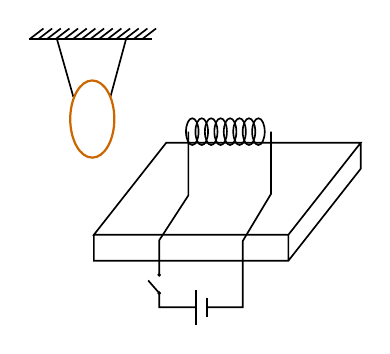
\begin{tikzpicture}[>=stealth,line width=.6pt]

\draw(-.65,2.88)--(.92,2.88);
\foreach \x in {-.63,-.52,...,.86}{\draw(\x,2.88)--++(.17,.13);}
\draw(-.29,2.88)--(-.08,2.14) (.59,2.88)--(.39,2.14);
\draw[orange!80!black,thick](.16,1.86)ellipse(.28 and .49);
\draw (.18,.39)--(2.65,.39)--(3.57,1.56)--(1.1,1.56)--cycle
 (.18,.39)--(.18,.06)--(2.65,.06)--(2.65,.39) (2.65,.06)--(3.57,1.23)--(3.57,1.56);
\draw(1.38,1.7)--(1.38,.89)--(1.01,.32)--(1.01,-.12) (2.43,1.7)--(2.43,.91)--(2.07,.31)--(2.07,-.53)--(1.62,-.53)
 (1.48,-.53)--(1.01,-.53)--(1.01,-.35);
\draw(1.01,-.35)--(.87,-.19);\fill(1.01,-.12)circle(.025) (1.01,-.35)circle(.025);
\foreach \x in {1.43,1.55,...,2.39}{\draw(\x,1.70)ellipse(.08 and .17);}
\draw(1.48,-.75)--(1.48,-.31) (1.62,-.65)--(1.62,-.41);

\end{tikzpicture}\end{center}
Замкнутое медное кольцо подвешено на длинных нитях вблизи катушки индуктивности, закрепленной на столе и подключенной к источнику постоянного тока (см. рис.). Первоначально электрическая цепь катушки разомкнута. Как будет двигаться кольцо при замыкании цепи? Ответ поясните, используя физические закономерности.
}{
\smallskip\noindent\textbf{Решение}\par
$1$.  При замыкании цепи катушки начинает изменяться поток вектора магнитной индукции через кольцо. По закону электромагнитной индукции в кольце возникает ЭДС индукции, появляется индукционный ток. В соответствии с правилом Ленца взаимодействие токов в кольце и в катушке приводит к тому, что кольцо отталкивается от катушки.
$2$.  Затем кольцо возвращается в исходное положение, так как ток в катушке достигает максимального значения, вследствие чего поток вектора магнитной индукции через кольцо становится постоянным. Индукционный ток в отсутствии ЭДС индукции затухает. Кольцо перестает отталкиваться от катушки.
$3$.  Индукционный ток в неподвижном кольце вблизи катушки с постоянным током равен нулю, магнитные свойства меди выражены слабо, поэтому, вернувшись в исходное положение равновесия, кольцо остается неподвижным.
}

% Source 8554: https://phys-ege.sdamgia.ru/problem?id=8554
\BankTask{8554}{
\begin{center}\begin{tikzpicture}[>=stealth,line width=.55pt]\draw(0,2.1)--(-.55,1.95)--(-.55,.42)--(0,.19)--(.53,.42)--(.53,1.95)--(0,2.1);\draw(0,2.1)..controls(1.65,2.05)and(2.26,1.53)..(2.2,1.2)..controls(2.02,.55)and(1.96,.88)..(2.17,1.24)..controls(2.5,1.73)and(2.5,.98)..(2.24,.73)..controls(1.55,.27)and(.64,.19)..(0,.19);\foreach \x/\i in {-.55/1,.53/2}{\draw[fill=white](\x,1.59)circle(.19);\draw(\x-.13,1.46)--(\x+.13,1.72) (\x-.13,1.72)--(\x+.13,1.46);\node[left]at(\x-.19,1.57){$\i$};}\node[above]at(0,2.1){А};\node[below]at(0,.19){Б};\draw[->](.5,2.9)--(1.27,2.9);\draw[<-](.5,3.19)--(1.27,3.19);\draw(.98,3.05)--(1.16,3.33) (1.16,3.05)--(.98,3.33);\node[left]at(.35,3.02){$I$};\draw(.5,2.52)--(1.27,2.52);\draw[fill=cyan!25](2.9,.9)rectangle(3.55,1.48)node[pos=.5]{$N$};\draw[fill=red!25](3.55,.9)rectangle(4.2,1.48)node[pos=.5]{$S$};\draw[->,orange!85!black](4.08,.64)--(3.02,.64);\begin{scope}[shift={(-0.55,0.94)},rotate=-90]\draw[fill=white](-.15,-.15)--(.11,0)--(-.15,.15)--cycle;\draw(.11,-.15)--(.11,.15);\end{scope}\begin{scope}[shift={(0.53,0.94)},rotate=90]\draw[fill=white](-.15,-.15)--(.11,0)--(-.15,.15)--cycle;\draw(.11,-.15)--(.11,.15);\end{scope}\begin{scope}[shift={(0.97,2.52)},rotate=0]\draw[fill=white](-.15,-.15)--(.11,0)--(-.15,.15)--cycle;\draw(.11,-.15)--(.11,.15);\end{scope}\end{tikzpicture}\end{center}Электрическая цепь состоит из двух лампочек, двух диодов и витка провода, соединенных как показано на рисунке. (Диод пропускает ток только в одном направлении, как показано в верхней части рисунка.) Какая из лампочек загорится, если к витку приближать северный полюс магнита? Ответ объясните, указав, какие явления и закономерности Вы использовали при объяснении.
}{
\smallskip\noindent\textbf{Решение}\par
$1$.  Загорится лампочка $2$.
$2$.  При приближении магнита к витку будет меняться магнитный поток сквозь виток, и в витке возникнет индукционный ток. Согласно правилу Ленца магнитное поле этого тока должно препятствовать движению магнита, поэтому выходящие из витка линии индукции этого поля будут направлены в сторону магнита. Для создания такого поля, согласно правилу «буравчика», индукционный ток в цепи, содержащей виток, должен быть направлен по часовой стрелке (если смотреть слева), а в цепи ламп  — от Б к А. Ток такого направления пропускает только диод на участке цепи лампочки $2$, она и будет гореть.
}

\end{document}
